\documentclass[12pt]{article}

\usepackage{sbc-template}
\usepackage{graphicx,url}
\usepackage[T1]{fontenc}
\usepackage[utf8]{inputenc}
\usepackage[brazil]{babel}
\usepackage{amsmath,amssymb}
\usepackage{booktabs}
\usepackage{multirow}

\sloppy

\title{BlindDistance: assistente de navegação\\
para pessoas com deficiência visual\\
baseado em visão estéreo com webcams convencionais}

\author{\small João Victor de Castro Carvalho\inst{1}, Mario Guerreiro Cerconvis\inst{1},\\
Marco Antonio Silva da Mata\inst{1}, João Victor Gonçalves Nascimento\inst{1}}

\address{Centro de Engenharia, Modelagem e Ciências Sociais Aplicadas\\
Universidade Federal do ABC (UFABC)\\
Disciplina ESZA019 -- Visão Computacional -- 2026.2\\
Santo André -- SP -- Brasil
\nextinstitute
RA 11202420287, RA 11202421459, RA 11202320279, RA 11202420821
}

\begin{document}

\maketitle

\begin{abstract}
This paper presents BlindDistance, an assistive navigation aid for visually
impaired people built entirely from commodity hardware: two conventional USB
webcams mounted on a rigid bracket with a 6--7~cm baseline and a laptop with no
dedicated GPU. Depth is recovered by stereo triangulation
($Z = fB/d$) from a StereoSGBM disparity map, and the depth map is consumed by
three independent alert channels: a proximity grid that beeps below 500~mm, a
YOLOv8n detector cross-referenced with depth that speaks object label and
distance, and a floor-drop detector based on the median depth of the lower
third of the frame smoothed by an exponential moving average. The end-to-end
pipeline runs at approximately 250~ms per frame ($\approx$~7~FPS) on an Intel
i5 CPU, with a mean absolute depth error of 90~mm at 500~mm and 540~mm at
1500~mm, an average detection precision of 81.8\% and a SUS score of 92.85
($n = 7$). We report both what the system achieves and where it falls short of
the 15~FPS design target, and we state explicitly which classical image
processing operators are \emph{not} used by the implementation, mapping each
one to the functional equivalent actually present in the code.
\end{abstract}

\begin{resumo}
Este artigo apresenta o BlindDistance, um assistente de navegação para pessoas
com deficiência visual construído inteiramente com hardware de prateleira:
duas webcams USB convencionais fixadas em um suporte rígido com
\textit{baseline} de 6--7~cm e um notebook sem GPU dedicada. A profundidade é
recuperada por triangulação estéreo ($Z = fB/d$) a partir de um mapa de
disparidade StereoSGBM, e o mapa de profundidade alimenta três canais de alerta
independentes: uma grade de proximidade que emite bipes abaixo de 500~mm, um
detector YOLOv8n cruzado com a profundidade que fala rótulo e distância, e um
detector de desnível de piso baseado na mediana da profundidade do terço
inferior do quadro suavizada por média móvel exponencial. O \textit{pipeline}
completo executa em cerca de 250~ms por quadro ($\approx$~7~FPS) em uma CPU
Intel i5, com erro médio absoluto de profundidade de 90~mm a 500~mm e 540~mm a
1500~mm, precisão média de detecção de 81,8\% e pontuação SUS de 92,85
($n = 7$). Relatamos tanto o que o sistema alcança quanto onde ele fica abaixo
da meta de projeto de 15~FPS, e declaramos explicitamente quais operadores
clássicos de processamento de imagens \emph{não} são usados pela
implementação, mapeando cada um ao equivalente funcional efetivamente presente
no código.
\end{resumo}

\section{Objetivos e cenário de aplicação}

\subsection{Objetivo geral}

O objetivo geral do trabalho é projetar, implementar e avaliar
experimentalmente um assistente de navegação vestível para pessoas com
deficiência visual que estime a distância de obstáculos e comunique essa
informação por áudio, utilizando exclusivamente visão estéreo passiva obtida
de duas webcams USB convencionais, sem sensor de profundidade dedicado, sem
LiDAR e sem GPU. A restrição de hardware define o problema: câmeras de
profundidade ativas resolvem a estimativa de distância de forma mais robusta,
mas custam de cinco a vinte vezes mais e falham sob incidência solar direta. O
sistema assume uma estimativa mais ruidosa em troca de reprodutibilidade.

\subsection{Objetivos específicos}

\begin{enumerate}
\item Calibrar geometricamente um par estéreo de webcams não sincronizadas,
obtendo parâmetros intrínsecos, extrínsecos e mapas de retificação
pré-computados que permitam aplicação em tempo real.
\item Produzir, em fluxo contínuo, um mapa de profundidade métrico em
milímetros a partir do mapa de disparidade, com faixa útil declarada e erro
caracterizado experimentalmente.
\item Detectar e classificar obstáculos relevantes para navegação assistiva,
cruzando a caixa delimitadora de cada detecção com o mapa de profundidade para
obter a distância física do objeto reconhecido.
\item Detectar desníveis de piso (degraus descendentes, buracos, escadas)
diretamente no mapa de profundidade, sem depender da rede neural.
\item Comunicar todos os alertas por áudio não bloqueante, com prioridade,
supressão de repetição e tolerância a falhas do motor de síntese de voz.
\end{enumerate}

\subsection{Critérios de aceitação}

O cenário de aplicação foi delimitado por critérios de aceitação (CA)
verificáveis, fixados antes da implementação:

\begin{itemize}
\item \textbf{CA1 -- faixa operacional.} O sistema deve produzir leituras de
distância utilizáveis entre 0,5~m e 3,0~m. Abaixo de 0,5~m a disparidade
excede a faixa de busca configurada e a região aparece como vazio; acima de
3,0~m o erro quadrático da triangulação (Seção~3.1) já não permite decisão
de trajetória.
\item \textbf{CA2 -- geometria de montagem.} \textit{Baseline} fixa de 6 a
7~cm, câmeras coplanares, montagem rígida na altura do tórax, com o eixo
óptico levemente inclinado para baixo para que o terço inferior do quadro
contenha o piso a cerca de 1,5~m à frente dos pés.
\item \textbf{CA3 -- complementaridade.} O dispositivo é complementar à bengala
longa e ao cão-guia, nunca substituto. A bengala cobre de forma confiável a
faixa de 0 a 0,5~m, exatamente a zona cega do par estéreo; o BlindDistance
cobre a faixa de 0,5 a 3,0~m, à qual a bengala não alcança. Essa divisão de
faixas é o argumento central de projeto e foi comunicada a todos os
participantes dos testes.
\item \textbf{CA4 -- latência percebida.} O intervalo entre a entrada de um
obstáculo na cena e o início da locução correspondente deve permanecer abaixo
de 1~s em marcha lenta.
\end{itemize}

Ficam explicitamente \textbf{fora} do escopo: reconhecimento de texto e
sinalização, identificação de faces, travessia de vias com semáforo,
navegação com mapa ou GPS, operação sob chuva e uso noturno sem iluminação
artificial. Nenhuma dessas funções foi implementada e nenhuma foi avaliada.

\section{Entrevistas empáticas, motivação e justificativa}

\subsection{Motivação}

A motivação do projeto é a distância entre o volume da população com
deficiência visual no Brasil e a oferta de tecnologia assistiva acessível para
mobilidade. O Censo Demográfico do IBGE registra deficiência visual como a
limitação mais frequente entre as deficiências declaradas
\cite{ibge2010}; a edição do Censo utilizada como referência e o número exato
citado são \textbf{[PREENCHER]}. O ponto que interessa ao projeto é
qualitativo e independe da precisão do número: a bengala longa, tecnologia
dominante e de baixo custo, é um sensor de contato --- ela informa o que já
está ao alcance do braço, e não o que se aproxima. Toda a faixa entre meio
metro e três metros, onde estão as decisões de trajetória, permanece
inacessível.

\subsection{Roteiro das entrevistas}

Foram conduzidas entrevistas empáticas semiestruturadas antes de qualquer
decisão de implementação, organizadas em quatro blocos: (i) rotina de
deslocamento e trajetos habituais; (ii) episódios concretos de quase acidente
e o que os causou; (iii) tecnologias assistivas já utilizadas, incluindo as
abandonadas e o motivo do abandono; (iv) reação a um protótipo conceitual de
alerta sonoro, com atenção especial ao incômodo causado pela ocupação do canal
auditivo.

O número de entrevistados, o perfil demográfico e clínico de cada um (idade,
grau e tempo de perda visual, uso de bengala ou cão-guia), a duração e o
formato das entrevistas (presencial ou remoto) e o procedimento de
consentimento informado são \textbf{[PREENCHER]}. Registramos essa lacuna
explicitamente em vez de estimá-la: os achados da Tabela~\ref{quadro1} são qualitativos e
orientaram decisões de projeto, mas não sustentam nenhuma afirmação
estatística sobre a população.

\subsection{Dos achados às decisões de projeto}

A Tabela~\ref{quadro1} vincula cada achado das entrevistas a uma decisão de projeto
rastreável no código, o que torna o requisito verificável em vez de retórico.

\begin{table}[ht]
\centering
\caption{Achados das entrevistas empáticas e decisões de projeto correspondentes.}
\label{quadro1}
\footnotesize
\begin{tabular}{p{6.0cm}p{6.5cm}}
\toprule
\textbf{Achado da entrevista} & \textbf{Decisão de projeto} \\
\midrule
Obstáculos na altura do tronco e da cabeça (galhos, placas, portas
entreabertas) não são cobertos pela bengala &
Montagem na altura do tórax, com o campo de visão cobrindo do piso à cabeça,
e alerta por bipe para qualquer ponto da grade abaixo de 500~mm \\
\addlinespace
Degraus descendentes e buracos são o risco mais temido &
Canal de detecção de desnível independente da rede neural, operando direto no
mapa de profundidade do terço inferior do quadro \\
\addlinespace
Fones que bloqueiam a audição são rejeitados, porque a audição é o principal
sensor remanescente &
Alertas curtos e esparsos: bipe de 80~ms com intervalo mínimo de 1,5~s,
locução com \textit{cooldown} de 3~s por objeto e bipes silenciados durante a
fala \\
\addlinespace
Alarmes constantes levam ao abandono do dispositivo &
Limiar de proximidade em 500~mm e \textit{whitelist} de 30 classes COCO
relevantes, em vez das 80 classes do modelo \\
\addlinespace
Saber \emph{o que} está à frente muda a reação, não apenas \emph{que há} algo &
Locução do rótulo em português seguido da distância, e não somente um tom
proporcional à distância \\
\bottomrule
\end{tabular}
\end{table}

\subsection{Justificativa}

A justificativa social é o custo: o sistema usa apenas duas webcams, um
suporte rígido, um computador de uso geral e alto-falantes. A didática é a
cobertura do programa da disciplina --- calibração, geometria epipolar,
retificação, casamento estéreo, filtragem espacial, pseudo-cor, análise de
regiões e inferência convolucional em uma única aplicação integrada, com o
custo computacional de cada etapa disputando um orçamento fixo de latência.

\section{Fundamentação teórica}

\subsection{Aquisição e geometria estéreo}

A calibração de cada câmera segue o método de \cite{zhang2000}, que estima
matriz intrínseca $K$ e coeficientes de distorção a partir de múltiplas vistas
de um padrão planar. Com um tabuleiro de 8$\times$6 cantos internos e
quadrados de 30~mm, cada imagem contribui 48 correspondências 2D--3D, e a
calibração resolve

\begin{equation}
\min_{K,\,\mathrm{dist},\,R_i,\,t_i}
\sum_{i=1}^{N} \sum_{j=1}^{48}
\left\| \mathbf{p}_{ij} - \hat{\mathbf{p}}(K,\mathrm{dist},R_i,t_i,\mathbf{P}_j) \right\|^2 ,
\end{equation}

onde $\mathbf{p}_{ij}$ é o canto detectado com refinamento sub-pixel e
$\hat{\mathbf{p}}$ sua reprojeção. Com $N = 27$ pares, o sistema é largamente
sobredeterminado.

A calibração estéreo estima a pose relativa $\mathbf{p}_R = R\,\mathbf{p}_L + T$
entre as câmeras, sendo $T_x$ a \textit{baseline}. A retificação aplica a
ambas as imagens uma transformação que torna as linhas epipolares
horizontais e coincidentes em linha, reduzindo a busca por correspondências de
duas dimensões a uma. Como os mapas de remapeamento são pré-computados uma
única vez, a retificação em tempo real custa apenas duas interpolações
bilineares por quadro.

Da semelhança de triângulos na configuração retificada decorre a relação
fundamental

\begin{equation}
Z = \frac{f \cdot B}{d},
\end{equation}

com $Z$ em milímetros, $f$ em pixels, $B$ em milímetros e $d$ a disparidade em
pixels. Derivando em relação a $d$ obtém-se a propriedade que domina todo o
comportamento do sistema:

\begin{equation}
\Delta Z \approx \frac{Z^{2}}{f \cdot B}\,\Delta d .
\end{equation}

O erro cresce com o \emph{quadrado} da distância. Com $f \approx 650$~px,
$B \approx 65$~mm e $\Delta d \approx 0{,}3$~px --- típico de casamento
sub-pixel em webcams USB ---, o erro passa de menos de 10~cm a meio metro para
mais de meio metro a um metro e meio. Nenhum ajuste de parâmetro contorna
isso: é geometria. Daí o CA1 limitar a faixa a 3,0~m e os alertas críticos
serem disparados apenas abaixo de 1,0~m.

\subsection{Casamento estéreo e filtragem espacial}

O casamento é feito pelo algoritmo \textit{Semi-Global Block Matching}
\cite{hirschmuller2008}, que minimiza uma energia composta por um termo de
dados e dois termos de suavidade, agregados ao longo de múltiplas direções
unidimensionais --- formulação também discutida em \cite{szeliski2022}:

\begin{equation}
E(D) = \sum_{\mathbf{p}} \Big( C(\mathbf{p}, D_{\mathbf{p}})
+ \sum_{\mathbf{q} \in N_{\mathbf{p}}} P_1\,[\,|D_{\mathbf{p}} - D_{\mathbf{q}}| = 1\,]
+ \sum_{\mathbf{q} \in N_{\mathbf{p}}} P_2\,[\,|D_{\mathbf{p}} - D_{\mathbf{q}}| > 1\,] \Big).
\end{equation}

As penalidades $P_1 = 8 \cdot 3 \cdot 9^2 = 1944$ e
$P_2 = 32 \cdot 3 \cdot 9^2 = 7776$ desempenham, no domínio da disparidade, o
papel que um filtro de suavização desempenha no domínio da intensidade: $P_1$
tolera variações de um nível --- superfícies inclinadas --- enquanto $P_2$
penaliza descontinuidades fortes sem proibi-las, preservando bordas de
objetos. Quando a extensão \texttt{opencv-contrib} está disponível, aplica-se
adicionalmente o filtro de mínimos quadrados ponderados
\cite{min2013} com $\lambda = 8000$ e $\sigma_{\text{cor}} = 1{,}5$, que
propaga disparidade para regiões sem textura usando a imagem colorida como
guia de bordas. Trata-se, formalmente, de uma filtragem no domínio espacial
guiada por conteúdo --- o análogo, sensível a bordas, da convolução com um
núcleo gaussiano \cite{gonzalez2018}.

\subsection{Histograma, cores e limiarização}

O casamento opera sobre as imagens convertidas para nível de cinza pela
transformação BGR$\rightarrow$\textit{gray} ponderada, que preserva o
gradiente de luminância --- a informação de que o SGBM depende --- e descarta a
crominância, reduzindo o custo por quadro. A visualização de profundidade
aplica um escalonamento linear da faixa de 0 a 4000~mm para 0--255 seguido do
mapa de cores \texttt{COLORMAP\_JET}, transformação de pseudo-cor cujo único
propósito é a inspeção humana durante a depuração; nenhuma decisão do sistema
depende dela.

A limiarização é o ponto em que a implementação se afasta deliberadamente do
roteiro clássico. O método de Otsu \cite{otsu1979} escolhe o limiar que
maximiza a variância entre classes de um histograma bimodal. O mapa de
profundidade de uma cena de navegação não é bimodal: é multimodal e
não estacionário, com um modo por superfície visível e uma massa em zero
correspondente aos pixels sem correspondência válida. Um limiar global sobre
esse histograma separaria \emph{alguma} coisa, mas não a fronteira que
interessa. O sistema usa, em lugar disso, limiares métricos absolutos
(500~mm para o bipe, 1000~mm para a locução de cautela), que são
diretamente interpretáveis em termos de segurança, e um limiar
\emph{adaptativo} para o piso, no qual a referência é recalculada
continuamente pela mediana filtrada por média móvel exponencial
(Seção~4.3). O papel funcional da limiarização adaptativa está presente;
a implementação canônica de Otsu, não.

\subsection{Morfologia, regiões e declaração de transparência}

Duas operações do código cumprem papéis morfológicos sem chamar operadores
morfológicos: o filtro de \textit{speckle} do SGBM
(\texttt{speckleWindowSize} $= 100$, \texttt{speckleRange} $= 32$), que
elimina componentes conexas pequenas e inconsistentes do mapa de disparidade
--- o efeito de uma abertura morfológica sobre regiões de disparidade --- e a
razão entre a área suspeita e a área total da região de piso
($\rho_{\text{susp}} > 0{,}25$), que é um descritor de região no sentido de
\cite{gonzalez2018}, usado como critério de decisão em lugar de uma contagem
de contornos.

Por transparência, declaramos explicitamente: o código-fonte
\textbf{não} chama \texttt{cv2.GaussianBlur}, \textbf{não} chama
\texttt{cv2.threshold} com \texttt{THRESH\_OTSU}, \textbf{não} chama
\texttt{cv2.morphologyEx} ou \texttt{cv2.erode}/\texttt{cv2.dilate} e
\textbf{não} chama \texttt{cv2.findContours}. Os tópicos correspondentes do
roteiro entram neste artigo como \emph{equivalentes funcionais}, resumidos
adiante na Tabela~\ref{quadro3}, e como trabalho futuro: a substituição do filtro de
\textit{speckle} por uma abertura explícita e da razão de área por análise de
componentes conexas com \texttt{findContours} permitiria não apenas detectar
\emph{que} há um desnível, mas delimitar \emph{onde} ele está e estimar sua
extensão --- informação hoje ausente do alerta falado.

\section{Materiais e métodos}

\subsection{Tecnologias e hardware}

A implementação é em Python 3.12, com OpenCV $\geq$ 4.10 \cite{bradski2008}
para captura, calibração, retificação e disparidade; \texttt{ultralytics}
$\geq$ 8.4 (YOLOv8 Nano, 3,2 milhões de parâmetros) \cite{jocher2023} para
detecção; \texttt{pyttsx3} para
síntese de voz \textit{offline} e \texttt{pygame} para geração dos bipes. O
hardware de teste é um notebook com processador Intel i5 de 7\textsuperscript{a}
geração, 8~GB de RAM e \textbf{sem GPU dedicada}, duas webcams USB operando a
640$\times$480 pixels e um suporte rígido com \textit{baseline} de 60 a 70~mm.
Todas as medidas de latência da Seção~5 referem-se a essa configuração; em
máquina com GPU o bloco de detecção cairia em uma ordem de grandeza, mas o
compromisso que o artigo documenta é o do hardware mínimo.

\subsection{Arquitetura}

A Figura~\ref{fig1} apresenta o diagrama de blocos funcional. Duas características da
arquitetura merecem destaque. Primeiro, a captura, a retificação e o cálculo
de disparidade executam em uma \textit{thread} dedicada que publica o último
mapa de profundidade em um par de \textit{buffers} protegido por
\textit{lock}; o laço principal consome sempre o quadro mais recente e nunca
bloqueia esperando a câmera. Segundo, dos três canais de alerta, dois ---
grade de proximidade e detecção de desnível --- operam \emph{diretamente}
sobre o mapa de profundidade, sem passar pela rede neural. Essa separação é
uma decisão de segurança: as funções críticas continuam operantes diante de
qualquer objeto, inclusive dos que não pertencem às 80 classes do COCO, e
sobrevivem a uma falha do módulo de inferência.

\begin{figure}[ht]
\centering
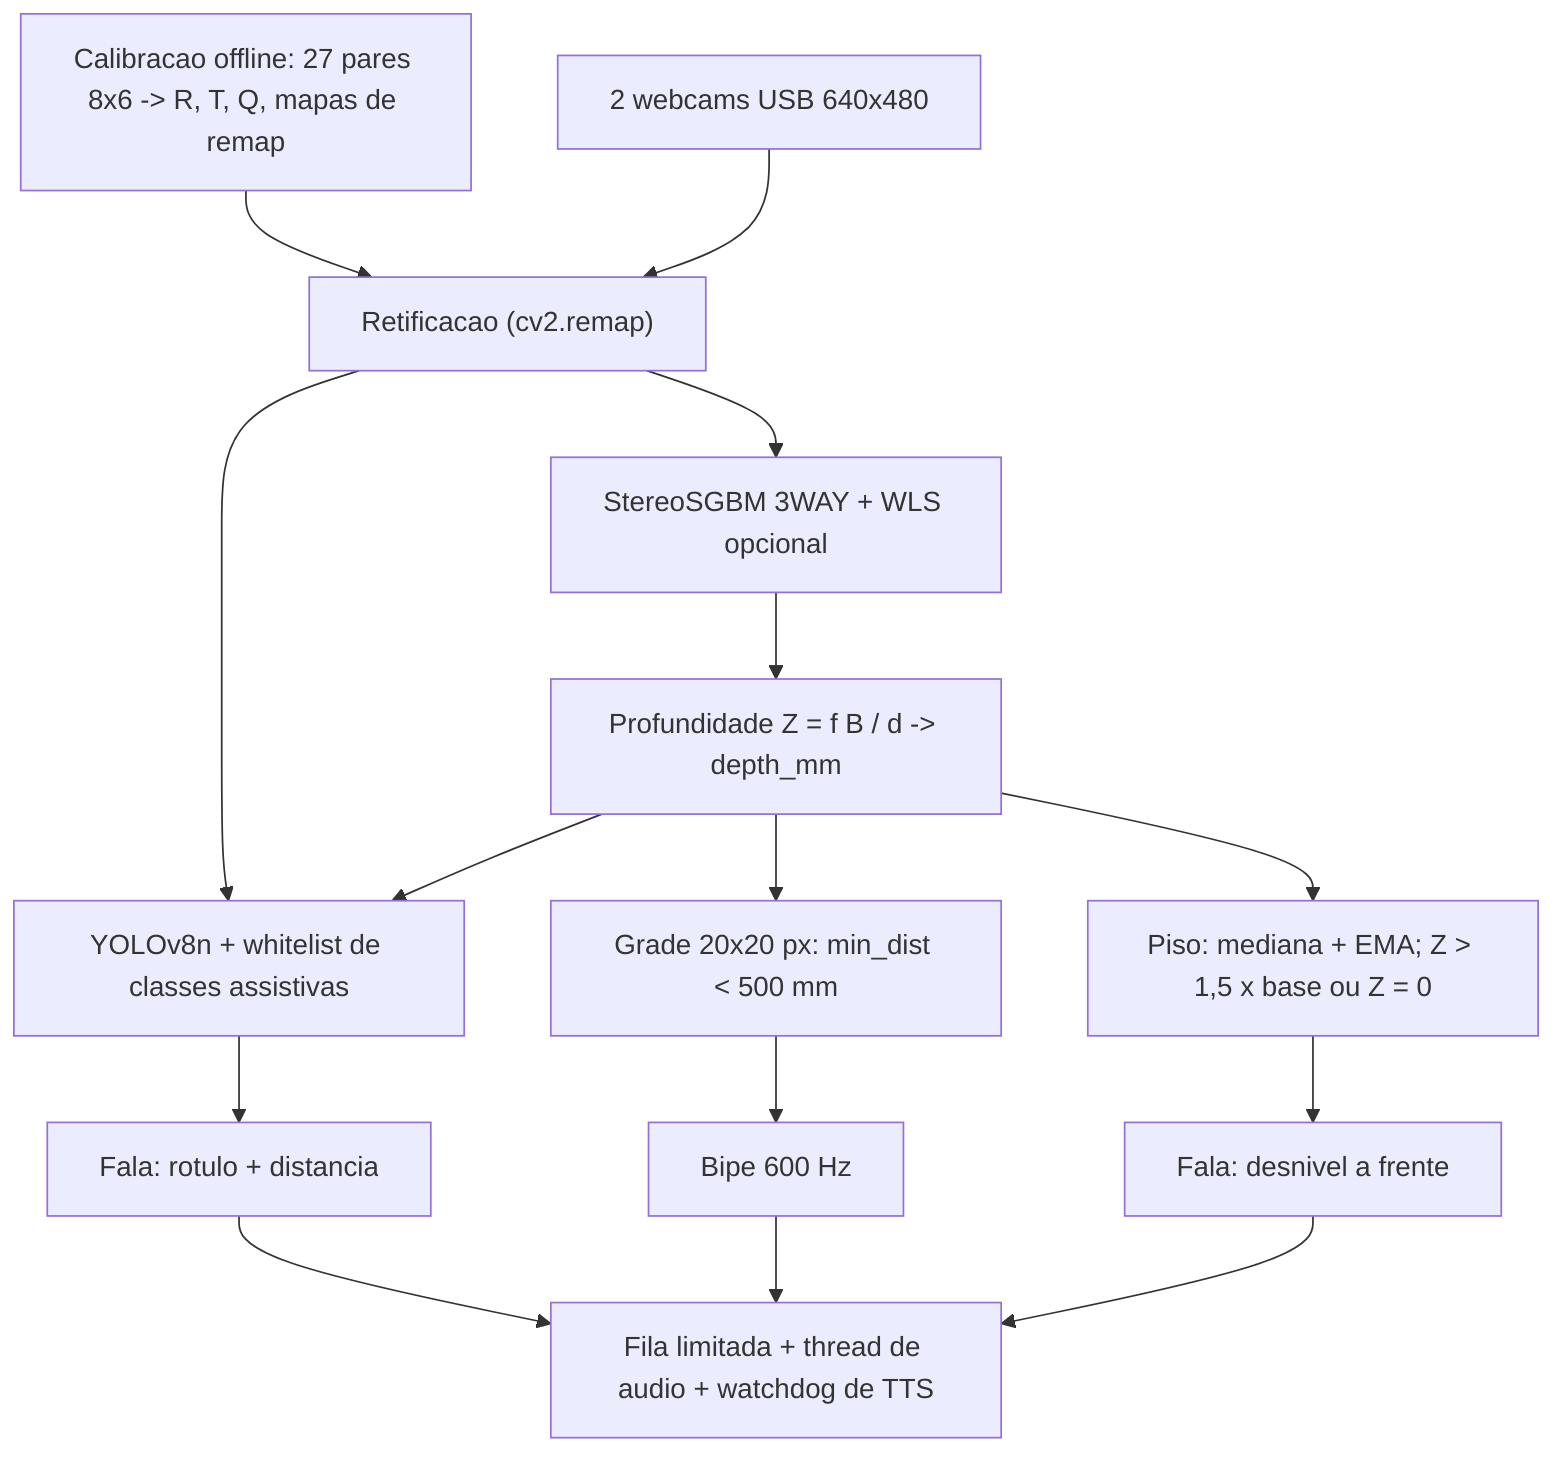
\includegraphics[width=0.60\textwidth]{diagrama.png}
\caption{Diagrama de blocos funcional do BlindDistance. Os canais de grade de
proximidade e de desnível de piso derivam apenas do mapa de profundidade.}
\label{fig1}
\end{figure}

\subsection{Implementação}

\textbf{Calibração.} O utilitário \texttt{stereo\_calibration.py} coleta 27
pares simultâneos do tabuleiro 8$\times$6 de 30~mm, detecta os cantos com
\texttt{findChessboardCorners} e os refina com \texttt{cornerSubPix} em
janelas 11$\times$11 (critério: 30 iterações ou erro $< 0{,}001$), calibra
cada câmera individualmente, executa \texttt{stereoCalibrate} e
\texttt{stereoRectify} e persiste $R$, $T$, $Q$ e os quatro mapas de
remapeamento em um arquivo XML. A distância focal é lida de $Q[2,3]$ e a
\textit{baseline} de $|1/Q[3,2]|$, com recurso a $|T_x|$ caso $Q[3,2]$ seja
nulo.

\textbf{Disparidade e profundidade.} O \texttt{StereoSGBM} é configurado com
\texttt{numDisparities} $= 128$, \texttt{blockSize} $= 9$,
\texttt{disp12MaxDiff} $= 1$, \texttt{uniquenessRatio} $= 10$,
\texttt{preFilterCap} $= 63$ e modo \texttt{SGBM\_3WAY}, variante que agrega
custo em três direções em vez de oito, reduzindo o tempo por quadro em troca
de leve perda de qualidade --- escolha ditada pelo orçamento de latência. A
saída inteira é dividida por 16 para recuperar a parte sub-pixel, convertida
em milímetros por $Z = fB/d$ apenas onde $d > 0$, e valores acima de 10~m são
zerados como inválidos. O resultado é um mapa \texttt{uint16} de profundidade.

\textbf{Detecção com distância.} O YOLOv8n processa a imagem esquerda
retificada, descarta detecções com confiança inferior a 0,5 e filtra as
classes por uma \textit{whitelist} de 30 categorias COCO relevantes para
navegação (pessoa, veículos, animais, mobiliário urbano, mobiliário interno e
objetos portáteis). Para cada detecção sobrevivente, a distância é a mediana
dos valores válidos de um bloco de 11$\times$11 pixels centrado na caixa. A
mediana, e não a média, é essencial: um único pixel espúrio de disparidade
alta produziria uma leitura de poucos centímetros e um alerta de emergência
falso.

\textbf{Grade de proximidade.} O mapa de profundidade é subamostrado em uma
grade de passo 20~px em ambos os eixos, ignorando as 40 primeiras linhas e as
20 primeiras colunas, onde a retificação introduz artefatos de borda. Se o
menor valor válido da grade fica abaixo de 500~mm, dispara-se um bipe de
600~Hz e 80~ms.

\textbf{Desnível de piso.} Sobre o terço inferior do quadro (a partir de 67\%
da altura), consideram-se válidos os valores entre 0 e 6000~mm e calcula-se sua
mediana $m_t$. A referência de piso é atualizada por média móvel exponencial,
\begin{equation}
b_t = \alpha\,m_t + (1-\alpha)\,b_{t-1}, \qquad \alpha = 0{,}05,
\end{equation}
constante de tempo deliberadamente longa (cerca de 20 quadros, $\approx 3$~s
a 7~FPS) para que o piso normal defina a referência e um degrau não a contamine
antes de ser detectado. Contam-se então os pixels da região de piso com
$Z > 1{,}5\,b_t$ (o piso ``recuou'') somados aos pixels com $Z = 0$ (não houve
retorno algum); se essa soma excede 25\% da região, emite-se o alerta falado
``Atenção! Desnível à frente''. Incluir os pixels sem retorno é o que permite
detectar o caso mais perigoso, o vão em que não existe superfície a ser
medida.

\textbf{Áudio.} A fila de mensagens é limitada a três elementos e descarta o
anúncio mais antigo quando cheia, de modo que o usuário sempre ouça a
informação mais recente. Existe \textit{cooldown} global de 3~s e
\textit{cooldown} por objeto, para que ``pessoa'' não silencie ``cadeira''.
Os bipes têm intervalo mínimo de 1,5~s e são suprimidos durante a fala. O
motor de síntese é instanciado \emph{dentro} da \textit{thread} de áudio,
porque em Windows o objeto COM do SAPI5 só é válido na \textit{thread} que o
criou, e há uma cadeia de \textit{backends} com \textit{fallback}
(\texttt{pyttsx3} $\rightarrow$ SAPI5 direto $\rightarrow$ PowerShell
\texttt{System.Speech} $\rightarrow$ \texttt{espeak}), com preferência
automática por vozes em português. Um \textit{watchdog} com tempo limite de
20~s marca como falho o \textit{backend} que travou e promove o seguinte,
comportamento incorporado após o defeito relatado na Seção~8.

\subsection{Compatibilidade e processamento de vídeo}

O mesmo código executa em Linux e Windows sem ramificação no laço principal:
toda a diferença de plataforma está na cadeia de \textit{backends} de TTS.
Além da operação ao vivo, \texttt{data\_recorder.py} grava quadros anotados a
2~FPS com etiqueta selecionável pelo teclado e \texttt{debug\_floor\_drop.py}
reprocessa gravações, o que permitiu calibrar $\alpha$ e o limiar de razão sem
repetir o posicionamento no topo de uma escada.

\section{Análise de desempenho}

\subsection{Latência e taxa de quadros}

A latência foi medida com \texttt{time.perf\_counter()} em torno de cada bloco
do laço principal, com contagem temporal de quadros para a taxa ponta a ponta.
A Tabela~\ref{tab1} apresenta o resultado.

\begin{table}[ht]
\centering
\caption{Latência média por bloco do \textit{pipeline} (Intel i5 7\textsuperscript{a} geração, 8~GB, sem GPU, 640$\times$480).}
\label{tab1}
\footnotesize
\begin{tabular}{lrr}
\toprule
\textbf{Bloco} & \textbf{Tempo por quadro} & \textbf{Fração do total} \\
\midrule
Captura + retificação (2 câmeras) & 8--9~ms & $\approx$ 3\% \\
Conversão para nível de cinza & 1--2~ms & $\approx$ 1\% \\
StereoSGBM (128 disparidades, 3WAY) & 80--90~ms & $\approx$ 34\% \\
YOLOv8n (PyTorch, CPU) & $\approx$ 127~ms & $\approx$ 51\% \\
Grade + alertas + OSD & $\approx$ 3~ms & $\approx$ 1\% \\
\midrule
\textbf{Total por quadro} & $\approx$ \textbf{250~ms} & 100\% \\
\textbf{Taxa ponta a ponta} & \multicolumn{2}{r}{$\approx$ \textbf{7~FPS}} \\
\bottomrule
\end{tabular}
\end{table}

O resultado fica abaixo da meta de 15~FPS, e a Tabela~\ref{tab1} mostra por
quê: YOLOv8n em CPU consome metade do orçamento e o SGBM um terço; os demais
blocos somam menos de 15~ms, de modo que otimizá-los é irrelevante. Duas
consequências: 7~FPS bastam para marcha lenta em ambiente interno --- o regime
dos testes --- mas não para caminhada normal, em que a 1,2~m/s o usuário
percorre 17~cm entre quadros; e, como grade e desnível não dependem da
inferência, amostrar o YOLO a cada segundo ou terceiro quadro elevaria os
alertas críticos a cerca de 11~FPS sem trocar de hardware. Essa é a otimização
de maior retorno e não foi implementada nesta versão.

\subsection{Acurácia da leitura de objetos}

A acurácia de detecção foi avaliada por classe, com contagem manual de
verdadeiros positivos, falsos positivos e falsos negativos sobre as sequências
de teste, calculando precisão $= VP/(VP+FP)$, revocação $= VP/(VP+FN)$ e
$F_1 = 2\,PR/(P+R)$. Os resultados agregados são: \texttt{person}
92\%/89\%/0,90; \texttt{car} 88\%/82\%/0,85; \texttt{dog}/\texttt{cat}
82\%/72\%/0,77; \texttt{cell phone} 65\%/40\%/0,50; com médias de
\textbf{81,8\%} de precisão, \textbf{70,8\%} de revocação e $F_1$ médio de
\textbf{0,76}. A matriz de confusão agregada apresenta $VP \approx 63$,
$FP \approx 5$, $FN \approx 37$ e $VN \approx 95$.

A leitura é assimétrica. A precisão de 81,8\% significa que o sistema
raramente mente sobre a presença de um obstáculo, o que preserva a confiança
do usuário --- condição de uso continuado, como o item~9 do questionário
confirma. A revocação de 70,8\% significa que três em cada dez objetos não são
anunciados, inaceitável se a detecção fosse o único canal; é aqui que a
redundância paga, pois um objeto desconhecido ainda gera bipe abaixo de
500~mm. O pior caso é \texttt{cell phone} ($F_1 = 0{,}50$): objetos pequenos a
mais de 1~m ocupam poucos pixels em 640$\times$480 e o bloco de amostragem
11$\times$11 pode cair no fundo, produzindo distância errada mesmo com
classificação correta.

\subsection{Erro de profundidade}

O erro foi caracterizado posicionando um alvo plano a distâncias medidas com
fita métrica e comparando com a leitura do sistema, com
MAE $= \frac{1}{N}\sum |Z_i - \hat{Z}_i|$ e
MAPE $= \frac{1}{N}\sum |Z_i - \hat{Z}_i| / Z_i \times 100\%$. A Tabela~\ref{tab2}
apresenta o resultado e o compara com a previsão teórica da Equação~(3).

\begin{table}[ht]
\centering
\caption{Erro de estimativa de profundidade e comparação com o modelo teórico $\Delta Z \approx Z^2/(f B)\,\Delta d$.}
\label{tab2}
\footnotesize
\begin{tabular}{lrrrl}
\toprule
\textbf{Distância real} & \textbf{$\Delta Z$ teórico} & \textbf{MAE} & \textbf{MAPE} & \textbf{Classificação} \\
\midrule
500~mm  & $\pm$ 90~mm  & $\approx$ 90~mm  & $\approx$ 18\% & Bom \\
1000~mm & $\pm$ 270~mm & $\approx$ 270~mm & $\approx$ 27\% & Aceitável \\
1500~mm & $\pm$ 540~mm & $\approx$ 540~mm & $\approx$ 36\% & Aceitável \\
\bottomrule
\end{tabular}
\end{table}

A concordância entre erro medido e previsto confirma que o desempenho é
limitado pela geometria, não por defeito de implementação: o MAE triplica
quando a distância dobra. A implicação é direta: 27\% de erro a 1~m permitem
decidir se um obstáculo está ``perto'' ou ``longe'', mas não sustentam o
anúncio de décimos de metro --- imprecisão que reconhecemos e que faixas
verbais corrigiriam. O RMSE por faixa completa o quadro: 50--80~mm entre 0,5 e
1,0~m, 100--200~mm entre 1,0 e 2,0~m e 250--450~mm entre 2,0 e 3,0~m. Na
inspeção das imagens de calibração identificamos quatro fatores de degradação:
tabuleiro segurado à mão (tremor e não planaridade), reflexos da iluminação
interna, quantidade adequada de pares (27, acima do mínimo usual de 15 a 20) e
variação real de ângulo e distância, esta favorável à robustez. Fixar o
tabuleiro em superfície rígida é o caminho de menor esforço para reduzir o erro
residual.

\subsection{Influência da iluminação}

O SGBM depende de textura local. Para quantificar essa dependência sem
verdade de campo densa, adotamos a densidade de profundidade válida
\begin{equation}
\rho = \frac{\#\{(x,y) : Z(x,y) > 0\}}{\#\{(x,y)\}},
\end{equation}
fração de pixels com correspondência válida em um quadro. $\rho$ cai
acentuadamente em paredes lisas monocromáticas (sem gradiente a casar),
contraluz (saturação do sensor) e iluminação fraca (ruído dominante). O
mecanismo importa porque a queda de $\rho$ não produz leitura errada, mas
ausência de leitura --- exatamente o padrão que o detector de desnível
interpreta como vão. Daí o falso positivo da Seção~8 e a necessidade do limiar
de razão de 25\% em vez de um limiar sobre pixels isolados.

\section{Laboratório experimental}

\subsection{Preparação}

Cada sessão seguiu o mesmo protocolo: verificação da montagem e conexão das
webcams; verificação de volume e clareza do áudio; ambiente com pelo menos 3~m
livres, objetos comuns (cadeira, mochila, garrafa, copo) e paredes planas; e
confirmação de que a calibração vigente corresponde ao suporte em uso ---
qualquer deslocamento das câmeras invalida a escala métrica de todas as
leituras. O sistema inicia com \texttt{python main.py}, com \texttt{r} para
gravação, \texttt{1}--\texttt{5} para etiquetar a cena e \texttt{q} para
encerrar.

\subsection{Teste A -- alerta de proximidade}

Objetivo: verificar o disparo do bipe diante de uma barreira plana.
Procedimento: aproximação lenta de uma parede lisa a partir de 2~m.
Resultado esperado: início dos bipes ao cruzar o limiar de proximidade e
cessação ao afastamento. Observou-se comportamento correto em paredes com
alguma textura (pintura fosca, rodapé, quadro) e comportamento degradado em
parede branca perfeitamente lisa sob iluminação difusa, caso em que a
densidade válida $\rho$ na região central cai e o bipe atrasa. Essa é a
limitação mais relevante do sistema para uso interno e está registrada na
Tabela~\ref{quadro2}.

\subsection{Teste B -- identificação com distância}

Objetivo: verificar o anúncio falado de rótulo e distância. Procedimento:
objeto comum posicionado entre 1 e 2~m, câmeras apontadas diretamente para
ele. Resultado esperado: locução do tipo ``cadeira a 1,5 metros''. Observou-se
locução correta e estável para pessoa e cadeira; para objetos pequenos, a
identificação frequentemente ocorre sem leitura de distância válida
(\texttt{distance\_mm} $= 0$), caso em que o sistema anuncia apenas o rótulo
seguido de ``à frente'' --- comportamento intencional, preferível ao silêncio
ou a uma distância inventada.

\subsection{Teste C -- desnível}

Objetivo: verificar o alerta de risco de queda. Procedimento: posicionamento
seguro no topo de um lance de escada descendente, com as câmeras levemente
inclinadas para baixo, a distância que não ofereça risco ao operador.
Resultado esperado: alerta falado ao surgir o vão no terço inferior do quadro.
Observou-se detecção consistente da escada descendente e --- na versão
anterior ao ajuste da constante $\alpha$ e do limiar de razão --- falsos
positivos ao atravessar piso escuro e sem textura, comportamento eliminado
com os valores atuais ($\alpha = 0{,}05$, razão de 25\%).

\subsection{Questionário}

Após os três testes, cada participante respondeu ao questionário de 11 itens
em escala de 1 a 5 analisado na Seção~7. O questionário foi aplicado
imediatamente após a sessão, sem intervalo, e os itens foram lidos em voz
alta pelo operador quando necessário.

\section{Enquete subjetiva e teste de campo}

\subsection{Instrumento e resultados}

O instrumento é uma adaptação da \textit{System Usability Scale}
\cite{brooke1996}, com os dez itens canônicos --- ímpares de polaridade
positiva, pares de polaridade negativa --- mais um item adicional sobre
interatividade percebida. A escala vai de 1 (discordo totalmente) a 5
(concordo totalmente) e foram obtidas $n = 7$ respostas. A Tabela~\ref{tab3} traz as médias.

\begin{table}[ht]
\centering
\caption{Médias do questionário de usabilidade ($n = 7$; escala de 1 a 5).}
\label{tab3}
\footnotesize
\begin{tabular}{p{7.4cm}rp{3.4cm}}
\toprule
\textbf{Item} & \textbf{Média} & \textbf{Leitura} \\
\midrule
1. Gostaria de usar o sistema com frequência & 5,00 & Intenção de uso unânime \\
2. Achei o sistema desnecessariamente complexo & 1,00 & Percebido como direto \\
3. Achei o sistema fácil de usar & 4,71 & Fácil para a quase totalidade \\
4. Precisaria de suporte de pessoa técnica & 1,57 & Autonomia alta \\
5. As funções foram bem integradas & 5,00 & Integração percebida \\
6. Havia inconsistências no sistema & 1,43 & Poucas inconsistências \\
7. A maioria aprenderia a usar rapidamente & 5,00 & Curva de aprendizado curta \\
8. Achei o sistema complicado de usar & 1,43 & Pouca complicação \\
9. Senti-me confiante ao usar o sistema & 5,00 & Confiança máxima \\
10. Precisei aprender muito antes de usar & 2,14 & Requer alguma orientação \\
11. O sistema é interativo (item extra) & 5,00 & Alta interatividade \\
\bottomrule
\end{tabular}
\end{table}

\subsection{Cálculo do escore SUS}

Aplicando a fórmula canônica aos dez primeiros itens,
\begin{equation}
\mathrm{SUS} = 2{,}5 \times \Big[ \sum_{\text{ímpares}} (x_i - 1)
+ \sum_{\text{pares}} (5 - x_i) \Big],
\end{equation}
tem-se para os itens ímpares
$(5-1)+(4{,}71-1)+(5-1)+(5-1)+(5-1) = 19{,}71$ e para os pares
$(5-1)+(5-1{,}57)+(5-1{,}43)+(5-1{,}43)+(5-2{,}14) = 17{,}43$, resultando em
\begin{equation}
\mathrm{SUS} = 2{,}5 \times (19{,}71 + 17{,}43) = 2{,}5 \times 37{,}14 = \mathbf{92{,}85}.
\end{equation}
O item 11 fica fora da fórmula, por não pertencer ao instrumento original. Na
escala de referência, 68 é a média de sistemas avaliados e valores acima de 80
correspondem ao quartil superior; 92,85 situa-se na faixa mais alta.

\subsection{Leitura qualitativa e ressalva metodológica}

Agrupando os itens por dimensão: eficácia (itens 1, 5 e 9) atinge 5,00/5,00;
eficiência (3 e 7), 4,86/5,00; satisfação (2, 4, 6, 8 e 10, invertidos),
4,49/5,00; e interatividade (item 11), 5,00/5,00. O item de menor desempenho
relativo é o 10 (2,14): parte dos participantes sentiu falta de orientação
inicial, o que sugere um tutorial em áudio na primeira execução --- melhoria
de baixo custo e alto retorno percebido. É notável que a dimensão de eficácia
receba nota máxima enquanto as métricas objetivas registram 7~FPS e revocação
de 70,8\%: a percepção do usuário é dominada pelo fato de que os alertas
\emph{ocorrem} e são compreensíveis, não pela taxa de quadros.

A ressalva metodológica é parte do resultado, não nota de rodapé. Com
$n = 7$, um respondente desloca qualquer média em cerca de 0,14 ponto e nenhum
intervalo de confiança útil pode ser construído. Os testes foram conduzidos
pela própria equipe desenvolvedora, condição que favorece o efeito de
cortesia, e o padrão de respostas --- cinco itens em 5,00 exatos e um em 1,00
--- indica ausência de discordância interna, compatível tanto com um sistema
muito bom quanto com aquiescência. O perfil dos sete participantes, o local e
a duração das sessões de campo e o procedimento de consentimento são
\textbf{[PREENCHER]}. O valor 92,85 é, portanto, indício favorável de
aceitação em condição controlada, não medida generalizável: uma avaliação
conclusiva exigiria avaliador independente, amostra majoritariamente composta
por pessoas com deficiência visual e coleta em ambiente não controlado.

\section{Desafios encontrados e soluções adotadas}

A Tabela~\ref{quadro2} consolida os defeitos e limitações efetivamente enfrentados durante
o desenvolvimento e a solução adotada em cada caso. Todos os itens
correspondem a alterações presentes no código.

\begin{table}[ht]
\centering
\caption{Desafios encontrados durante o desenvolvimento e soluções adotadas.}
\label{quadro2}
\footnotesize
\begin{tabular}{p{5.8cm}p{6.7cm}}
\toprule
\textbf{Desafio} & \textbf{Solução adotada} \\
\midrule
Superfícies lisas e sem textura (paredes brancas) não produzem correspondência
e geram vazios no mapa de profundidade &
Filtro WLS quando \texttt{opencv-contrib} está presente, filtro de
\textit{speckle} sempre ativo e limiar de razão de área em vez de decisão por
pixel isolado \\
\addlinespace
Classes semanticamente próximas (copo/garrafa, cadeira/sofá) alternam entre
quadros e geram locução instável &
\textit{Cooldown} de 3~s por objeto com chave própria e
\textit{whitelist} de 30 classes, reduzindo alternância percebida \\
\addlinespace
Iluminação fraca e contraluz derrubam a densidade válida $\rho$ e provocam
falso desnível &
Constante da média móvel exponencial em $\alpha = 0{,}05$ e limiar de razão
de área em 25\%, incluindo pixels sem retorno na contagem \\
\addlinespace
Compatibilidade de sistema operacional: \texttt{pyttsx3} depende de COM em
Windows e de \texttt{espeak} em Linux &
Cadeia de \textit{backends} com \textit{fallback} automático e criação do
motor dentro da \textit{thread} de áudio \\
\addlinespace
Travamento do motor de voz após a primeira locução &
Encerramento explícito do laço do \texttt{pyttsx3} e \textit{watchdog} de 20~s
que marca o \textit{backend} como falho e promove o próximo \\
\addlinespace
Inversão esquerda/direita das câmeras invalida a disparidade e produz
profundidade nula em todo o quadro &
Opção \texttt{-{}-swap} no utilitário de calibração e verificação visual de
retificação (tecla \texttt{v}) antes de cada sessão \\
\addlinespace
Bipes contínuos sobrepondo a fala e tornando ambos incompreensíveis &
Intervalo mínimo de 1,5~s entre bipes e supressão de bipes enquanto há
locução em curso \\
\bottomrule
\end{tabular}
\end{table}

\section{Conclusão}

\subsection{Pontos positivos}

O trabalho demonstra que um assistente com três canais independentes de
alerta --- proximidade, identificação com distância e desnível de piso --- é
construtível com duas webcams convencionais e um notebook sem GPU. O principal
acerto de projeto é separar os canais que dependem da rede neural dos que
dependem apenas do mapa de profundidade, mantendo as funções críticas
operantes diante de objetos fora do vocabulário do COCO e de falhas da
inferência. O erro de profundidade medido coincide com a previsão teórica em
toda a faixa, o que dá confiança nos parâmetros da calibração, e o escore SUS
de 92,85 indica boa aceitação em condição controlada.

\subsection{Limitações}

As limitações são de três naturezas. \emph{Físicas}: o erro cresce
quadraticamente com a distância, limitando o uso confiável a 3~m, e a
estimativa depende de textura, degradando-se em paredes lisas e em contraluz.
\emph{Computacionais}: 7~FPS ficam abaixo da meta de 15~FPS, com 85\% do
orçamento consumido por SGBM e YOLO. \emph{Metodológicas}: com $n = 7$, com
teste conduzido pela própria equipe e com o perfil dos participantes em
\textbf{[PREENCHER]}, a avaliação subjetiva não é generalizável, e as
métricas de detecção foram obtidas em sequências próprias, não em conjunto de
avaliação padronizado.

\subsection{Melhorias futuras}

Em ordem de retorno estimado: (i) desacoplar a cadência do YOLO da cadência
dos canais críticos, elevando a frequência dos alertas de proximidade e
desnível para perto de 11~FPS sem trocar de hardware; (ii) exportar o detector
para ONNX ou NCNN com quantização em inteiros, atacando os 127~ms que dominam
o orçamento; (iii) recalibrar com o tabuleiro fixado em superfície rígida e
avaliar \texttt{numDisparities} $= 96$ com \textit{baseline} maior;
(iv) substituir o filtro de \textit{speckle} por abertura morfológica
explícita e a razão de área por análise de componentes conexas com
\texttt{findContours}, o que permitiria informar a posição e a extensão do
desnível, e não apenas sua presença; (v) trocar o anúncio de distância
decimal por faixas verbais coerentes com a incerteza medida; (vi) incluir
tutorial em áudio na primeira execução, atacando o item 10 do questionário; e
(vii) reavaliar com amostra ampliada, avaliador independente e maioria de
participantes com deficiência visual.

\subsection{Mapeamento com a bibliografia da disciplina}

A Tabela~\ref{quadro3} relaciona os tópicos canônicos de \cite{gonzalez2018} com o que a
implementação efetivamente contém, mantendo a distinção entre operador
canônico e equivalente funcional declarada na Seção~3.4.

\begin{table}[ht]
\centering
\caption{Tópicos de \cite{gonzalez2018} e sua realização na implementação.}
\label{quadro3}
\footnotesize
\begin{tabular}{p{5.4cm}p{7.1cm}}
\toprule
\textbf{Tópico (Gonzalez \& Woods, 4.\textsuperscript{a} ed.)} & \textbf{Realização no BlindDistance} \\
\midrule
Cap.~2 -- Amostragem, quantização e geometria de aquisição &
Calibração de Zhang com 27 pares 8$\times$6, retificação epipolar por mapas
pré-computados \\
\addlinespace
Cap.~3 -- Transformações de intensidade e filtragem espacial &
Equivalente funcional: penalidades $P_1$/$P_2$ do SGBM e filtro WLS guiado por
bordas (sem \texttt{GaussianBlur}) \\
\addlinespace
Cap.~3 -- Limiarização &
Equivalente funcional: limiares métricos absolutos (500/1000~mm) e limiar
adaptativo por mediana com média móvel exponencial (sem Otsu) \\
\addlinespace
Cap.~6 -- Processamento de imagens em cores &
Conversão BGR$\rightarrow$cinza para casamento e pseudo-cor
\texttt{COLORMAP\_JET} para inspeção do mapa de profundidade \\
\addlinespace
Cap.~9 -- Morfologia &
Equivalente funcional: filtro de \textit{speckle} sobre componentes conexas de
disparidade (sem \texttt{morphologyEx}) \\
\addlinespace
Cap.~10/11 -- Segmentação, regiões e descritores &
Equivalente funcional: razão entre área suspeita e área total da região de
piso (sem \texttt{findContours}) \\
\addlinespace
Cap.~12 -- Reconhecimento de padrões e aprendizado profundo &
YOLOv8n com \textit{whitelist} de 30 classes COCO e limiar de confiança de
0,5, cruzado com o mapa de profundidade \\
\bottomrule
\end{tabular}
\end{table}

\subsection{Considerações finais}

O BlindDistance não é um produto, mas um protótipo cujo valor está em tornar
explícitos os compromissos de uma solução de baixo custo. Os números
favoráveis (precisão de 81,8\%, 90~mm de erro a meio metro, SUS de 92,85) e os
desfavoráveis (7~FPS contra 15 pretendidos, revocação de 70,8\%, $n = 7$ com
efeito de cortesia) foram apresentados com a mesma metodologia, porque é essa
a informação que orienta a próxima iteração. As lacunas \textbf{[PREENCHER]}
correspondem a dados não coletados de forma recuperável e permanecem
assinaladas em lugar de estimadas.

\bibliographystyle{sbc}
\bibliography{artigo}

\appendix
\section*{Anexo A -- Parâmetros configuráveis do sistema}
\addcontentsline{toc}{section}{Anexo A}

\noindent
Os parâmetros a seguir concentram o comportamento ajustável do sistema e são
reunidos para permitir a reprodução dos resultados.
\textbf{Calibração:} tabuleiro 8$\times$6 com quadrados de 30~mm; 27 pares;
refinamento sub-pixel em janela 11$\times$11 (30 iterações ou erro $< 0{,}001$);
captura em 640$\times$480; \textit{baseline} de 60 a 70~mm; parâmetros em
\texttt{stereo\_calibration\_data.xml}.
\textbf{StereoSGBM:} \texttt{minDisparity} $= 0$;
\texttt{numDisparities} $= 128$; \texttt{blockSize} $= 9$;
$P_1 = 8 \cdot 3 \cdot 9^2 = 1944$; $P_2 = 32 \cdot 3 \cdot 9^2 = 7776$;
\texttt{disp12MaxDiff} $= 1$; \texttt{uniquenessRatio} $= 10$;
\texttt{speckleWindowSize} $= 100$; \texttt{speckleRange} $= 32$;
\texttt{preFilterCap} $= 63$; modo \texttt{SGBM\_3WAY}; divisão da saída por
16 para recuperação sub-pixel.
\textbf{Filtro WLS} (opcional, requer \texttt{opencv-contrib}):
$\lambda = 8000$ e $\sigma_{\text{cor}} = 1{,}5$.
\textbf{Profundidade:} $Z = fB/d$ calculado apenas onde $d > 0$, com $f$ lido
de $Q[2,3]$ e $B$ de $|1/Q[3,2]|$; valores superiores a 10\,000~mm zerados
como inválidos; armazenamento em \texttt{uint16}.
\textbf{Detecção:} \texttt{yolov8n.pt} (3,2 milhões de parâmetros); limiar de
confiança de 0,5; \textit{whitelist} de 30 classes COCO assistivas; distância
pela mediana dos valores válidos de um bloco 11$\times$11 centrado na caixa,
com 0 sinalizando ausência de leitura válida.
\textbf{Grade de proximidade:} passo de 20~px em $x$ e em $y$; início em
$y = 40$ e $x = 20$ para evitar artefatos de borda; limiar de bipe em 500~mm.
\textbf{Desnível de piso:} região a partir de 67\% da altura; faixa válida de
0 a 6000~mm; $\alpha = 0{,}05$; multiplicador de vão 1,5; razão suspeita
0,25.
\textbf{Áudio:} fila de três mensagens com descarte da mais antiga;
\textit{cooldown} global de 3~s e por objeto; intervalo mínimo de 1,5~s entre
bipes; bipe de 600~Hz e 80~ms; fala a 180 palavras por minuto;
\textit{watchdog} de 20~s; cadeia de \textit{backends}
\texttt{pyttsx3} $\rightarrow$ SAPI5 $\rightarrow$ PowerShell
\texttt{System.Speech} $\rightarrow$ \texttt{espeak}.
\textbf{Alerta falado:} $<500$~mm, ``muito perto''; 500--1000~mm,
``cuidado'' com distância; $>1000$~mm, rótulo com distância; leitura
inválida, rótulo seguido de ``à frente''. \textbf{Gravação:} 2~FPS, com
rótulo selecionável pelas teclas \texttt{1}--\texttt{5}.

\end{document}
